\chapter{Laporan Aplikasi Akademik}
\section{Membuat workspace}
Berikut adalah langkah-langkah membuat workspace
\begin{itemize}
    \item Pertama yaitu untuk kita harus membuat workspace, jika sudah mempunyai account apex oracle langsung saja request workspace.
    \begin{figure}[!htbp]
        \centering
        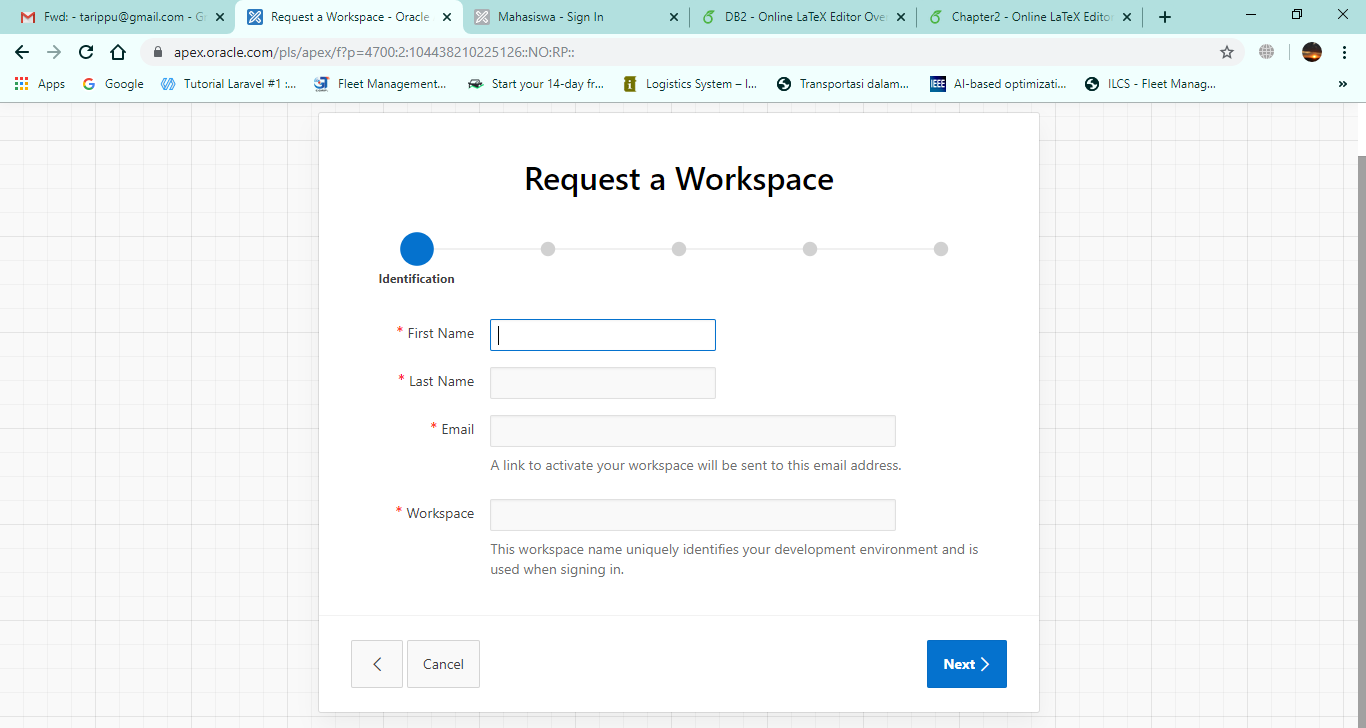
\includegraphics[width=10cm]{figures/work1.PNG}
        \caption{Workspace}
    \end{figure}
    
    \item Masukkan data-data identification yang diminta yaitu firstname, lastname, email dan nama workspace yg akan dibuat.
    \begin{figure}[!htbp]
        \centering
        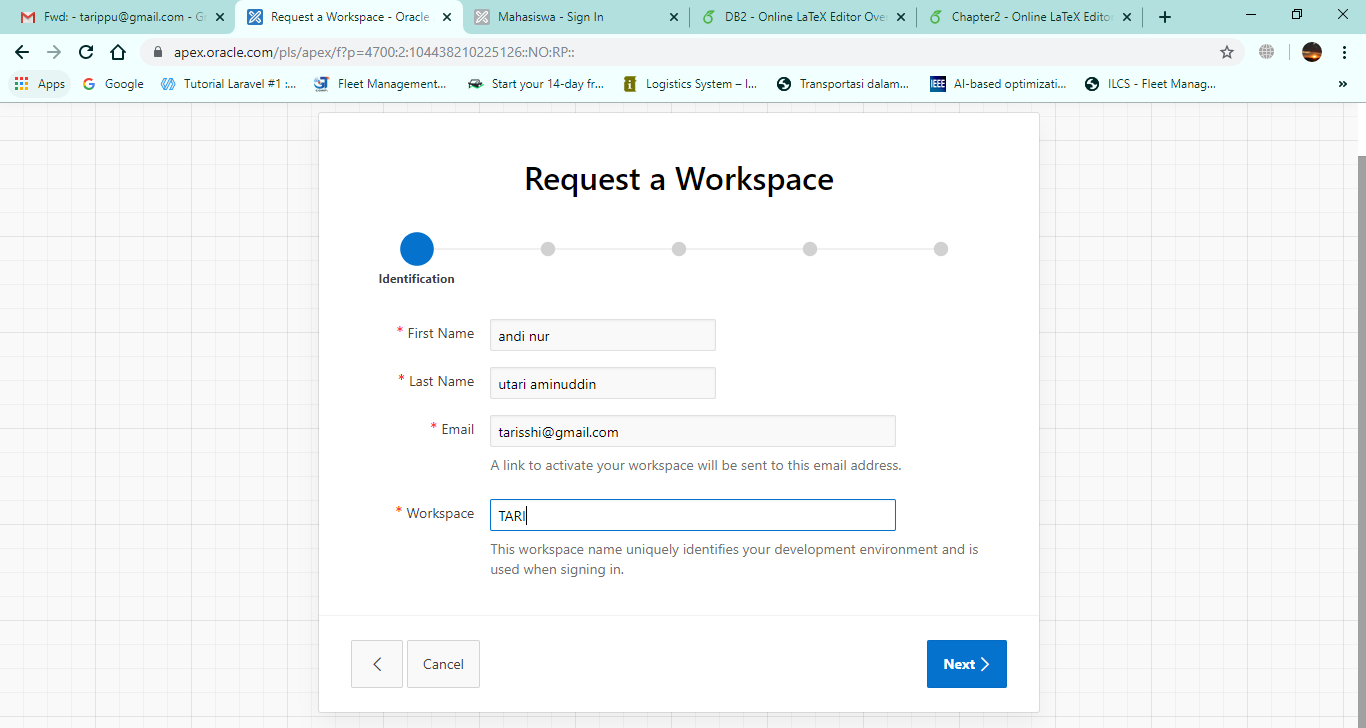
\includegraphics[width=10cm]{figures/work2.PNG}
        \caption{Identification}
    \end{figure}
    
    \newpage
    
    \item Pilih YES untuk kedua jawaban survey.
    \begin{figure}[!htbp]
        \centering
        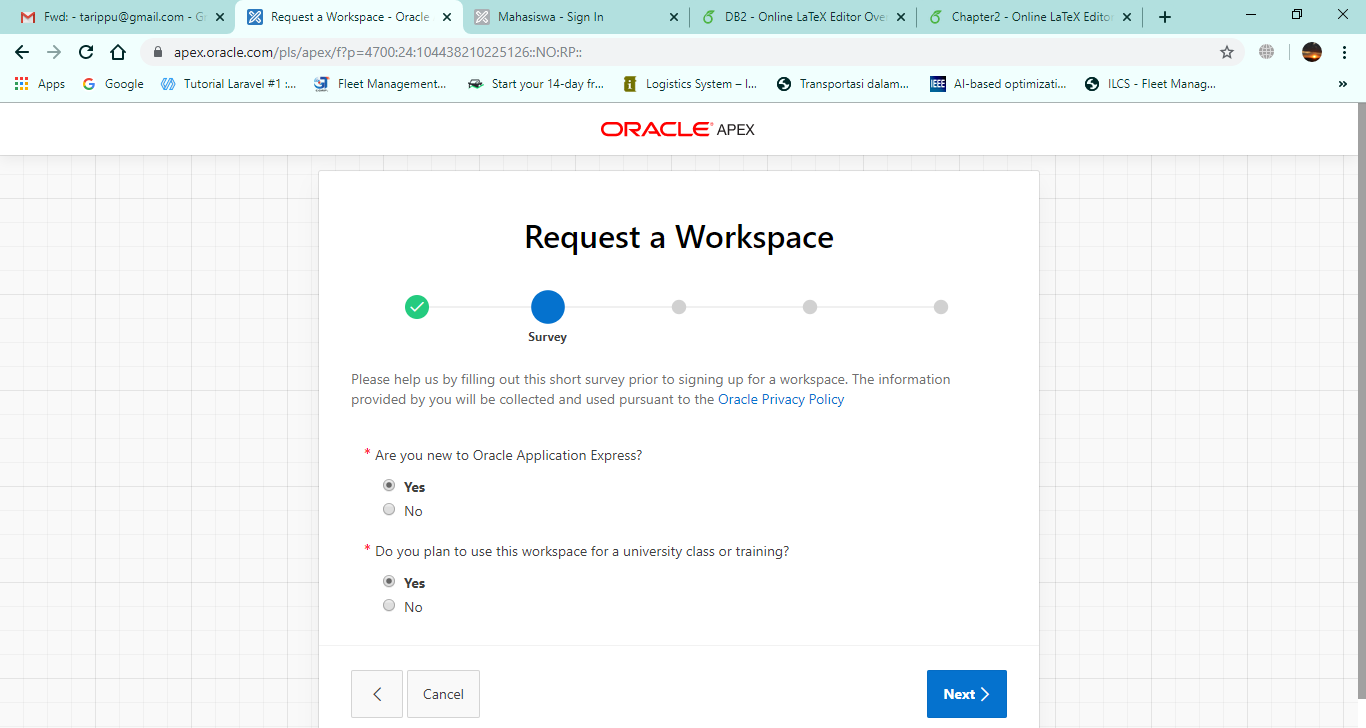
\includegraphics[width=10cm]{figures/work3.PNG}
        \caption{Survey}
    \end{figure}
    
    \item Isi Justification dengan alasan menggunakan apex.
    \begin{figure}[!htbp]
        \centering
        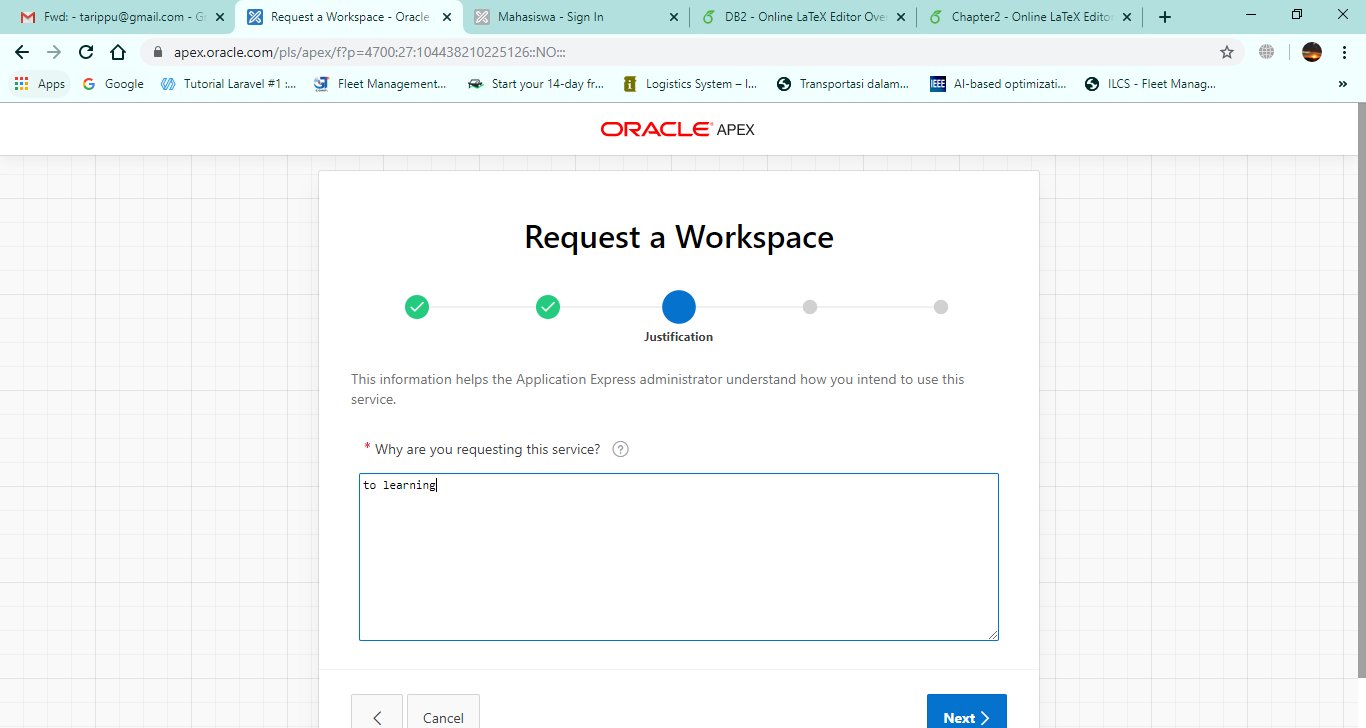
\includegraphics[width=10cm]{figures/work4.PNG}
        \caption{Justification}
    \end{figure}
    
    \newpage
    
    \item Klik i accept the terms untuk perintah agreement
    \begin{figure}[!htbp]
        \centering
        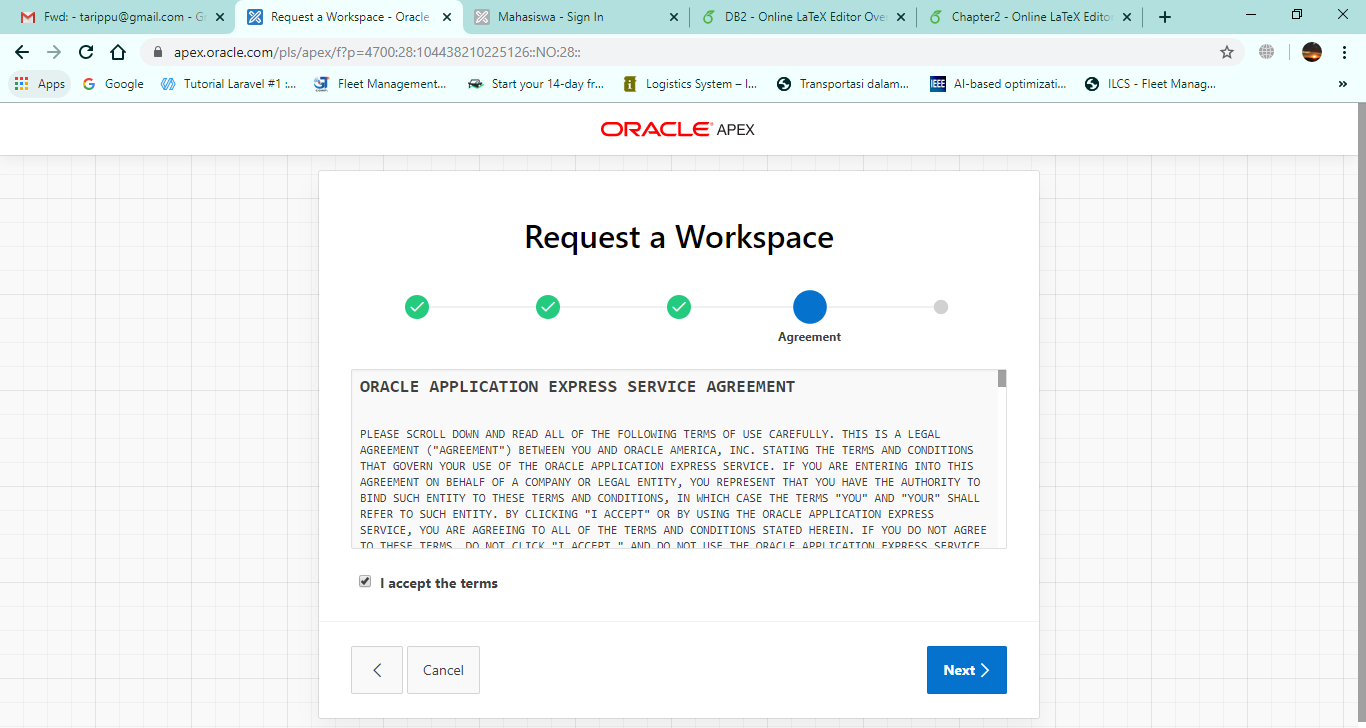
\includegraphics[width=10cm]{figures/work5.PNG}
        \caption{Agreement}
    \end{figure}
    
    \item Setelah melewati semua tahap, tahap terkahir yaitu confirmation. Klik Submit request.
    \begin{figure}[!htbp]
        \centering
        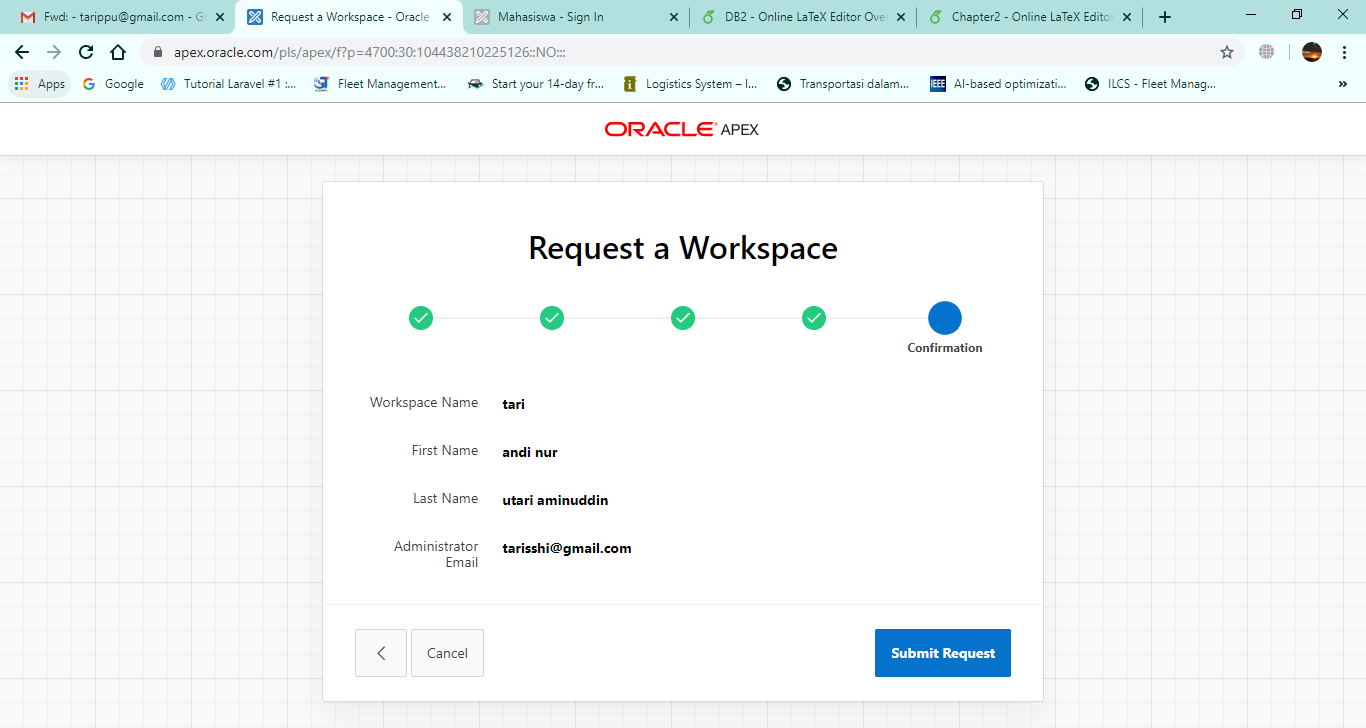
\includegraphics[width=10cm]{figures/work6.PNG}
        \caption{Buka aplikasi apex}
    \end{figure}
    
    \newpage
    
    \item Workspace request berhasil dibuat.
    \begin{figure}[!htbp]
        \centering
        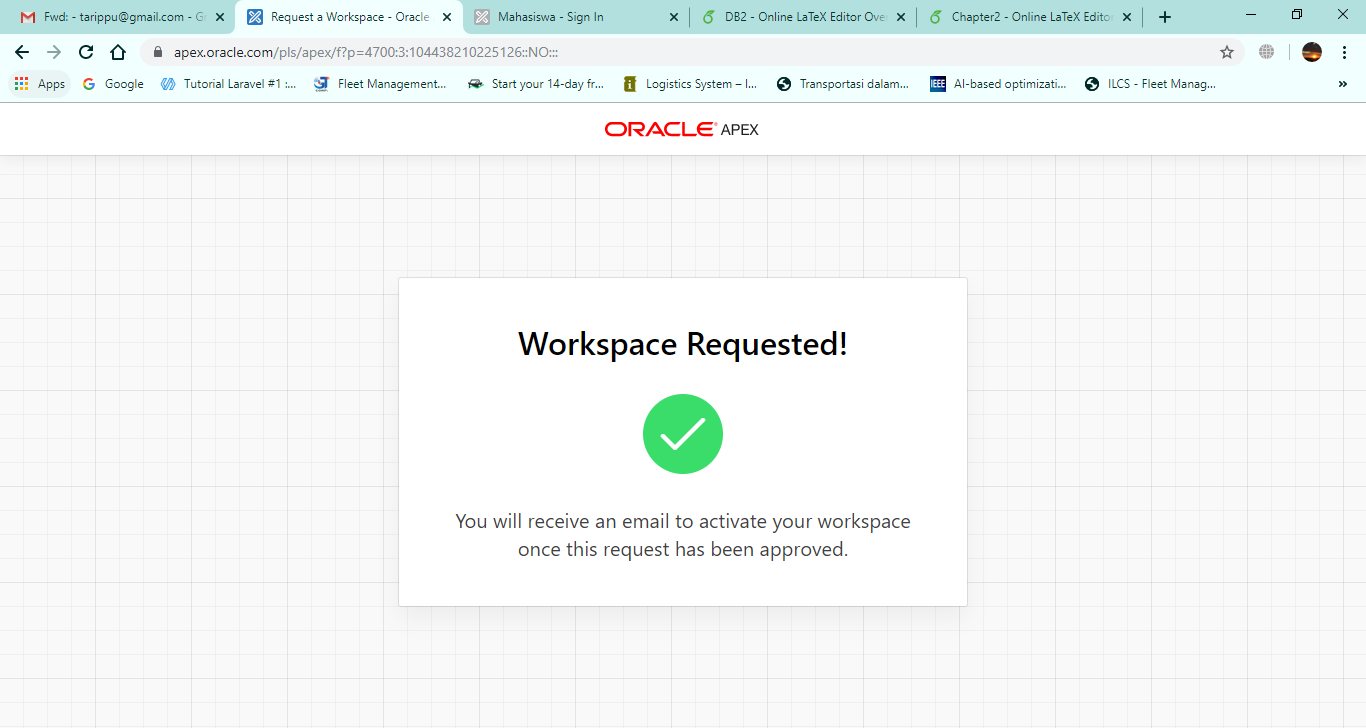
\includegraphics[width=10cm]{figures/workberhasil.PNG}
        \caption{Buka aplikasi apex}
    \end{figure}
\end{itemize}


\section{Membuat aplikasi akademik}
Berikut adalah langkah-langkah pembuatan aplikasi akademik menggunakan APEX

\begin{itemize}
    \item Untuk membuat aplikasi akademik kita harus mempunyai data yang sudah di normalisasikan terlebih dahulu, data yang akan dibuatkan aplikasinya yaitu data mahasiswa.
    
    \item Buka aplikasi apex atau link berikut\\ https://apex.oracle.com/pls/apex/f?p=4550:1:16642045919295:::::
    \begin{figure}[!htbp]
        \centering
        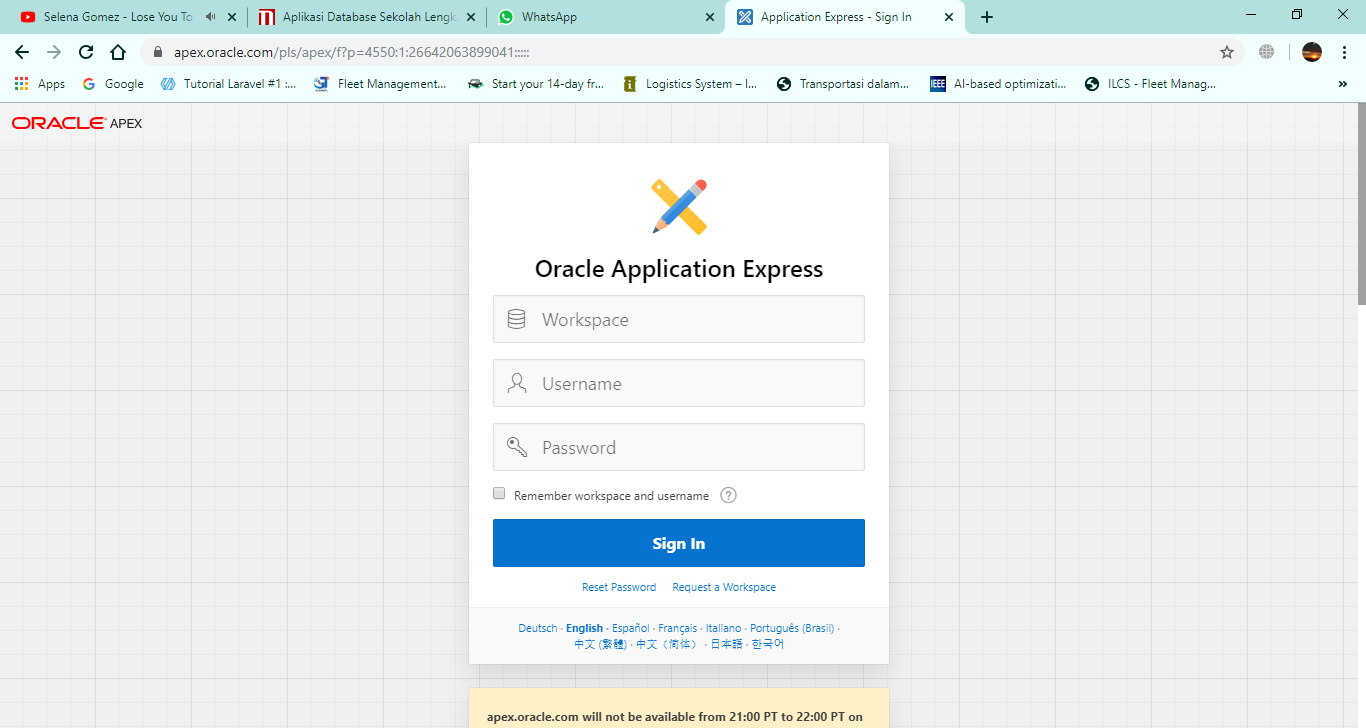
\includegraphics[width=10cm]{figures/1.PNG}
        \caption{Buka aplikasi apex}
    \end{figure}
    
    \newpage
    
    \item Login dengan memasukkan workspace, username, dan password yang sudah dibuat.
    \begin{figure}[!htbp]
        \centering
        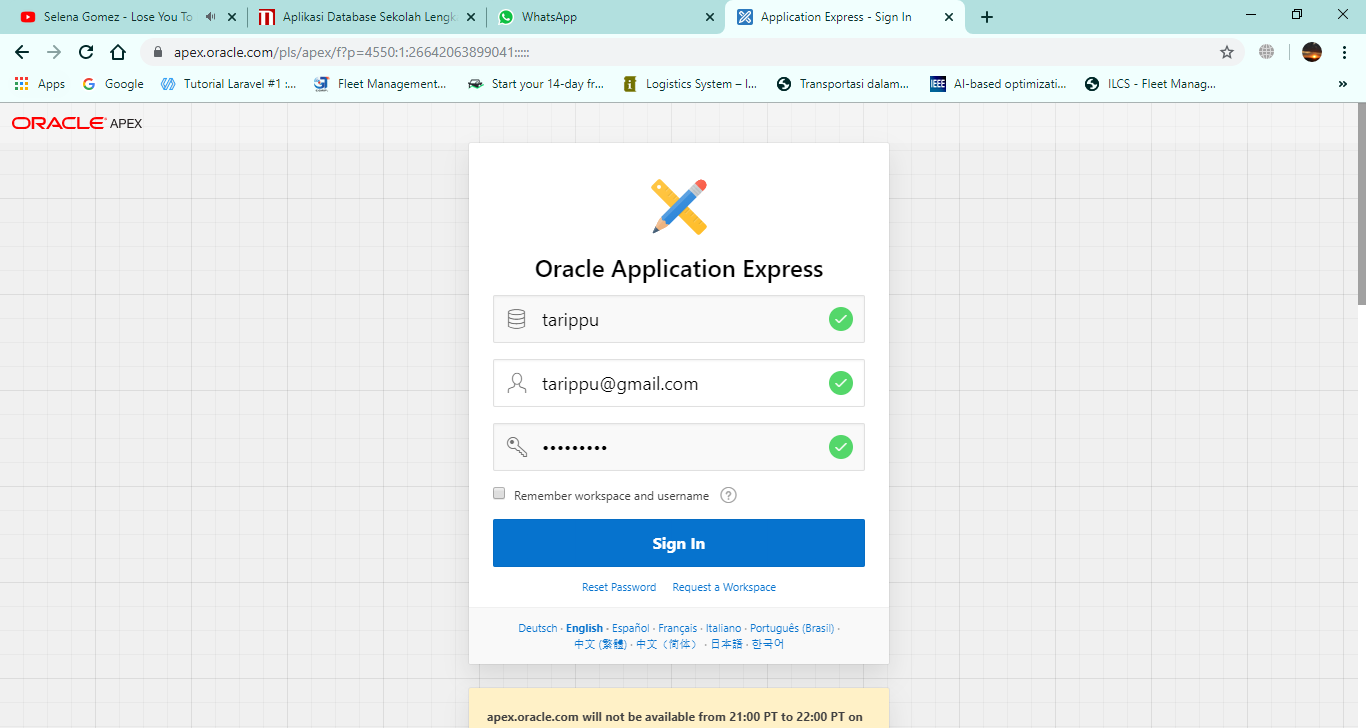
\includegraphics[width=10cm]{figures/2.PNG}
        \caption{Login}
    \end{figure}
    
    \item Setela berhasil login akan muncul tampilan seperti berikut. Klik App Builder.
    \begin{figure}[!htbp]
        \centering
        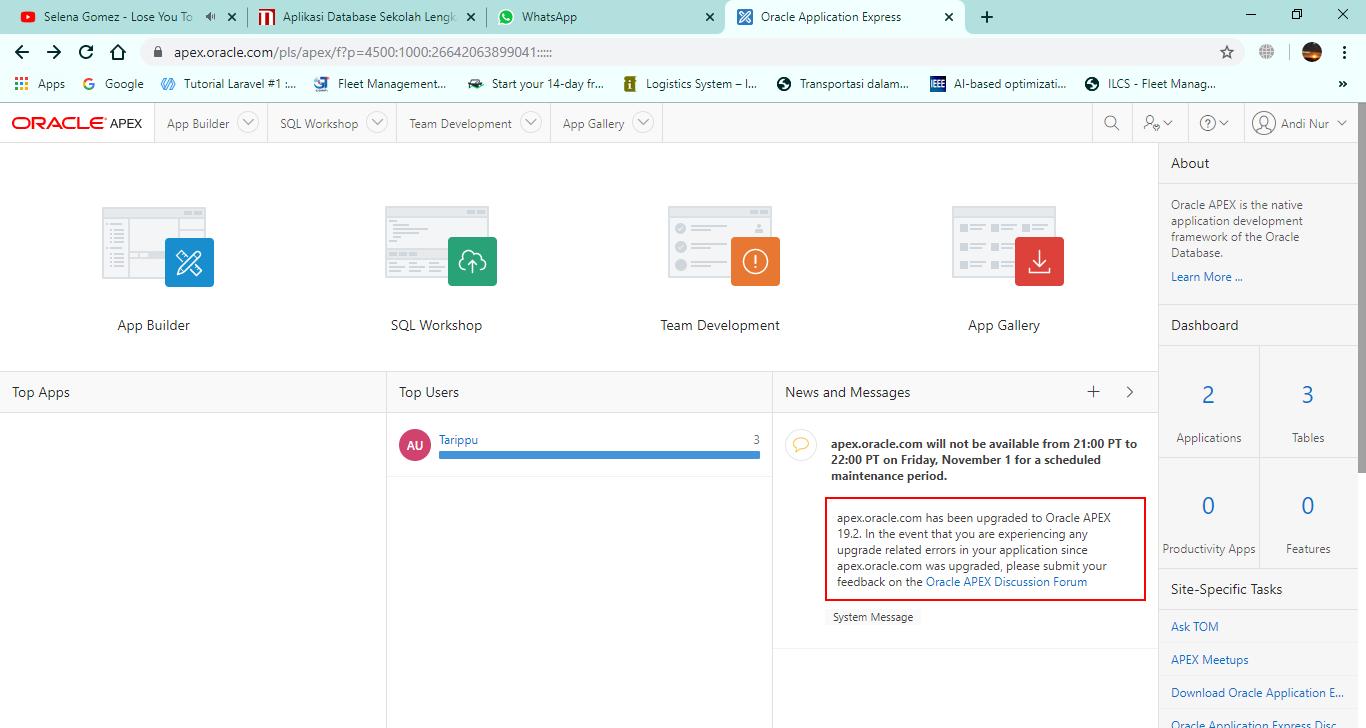
\includegraphics[width=10cm]{figures/3.PNG}
        \caption{App Builder}
    \end{figure}
    
    \newpage
    
    \item Lalu pilih create
    \begin{figure}[!htbp]
        \centering
        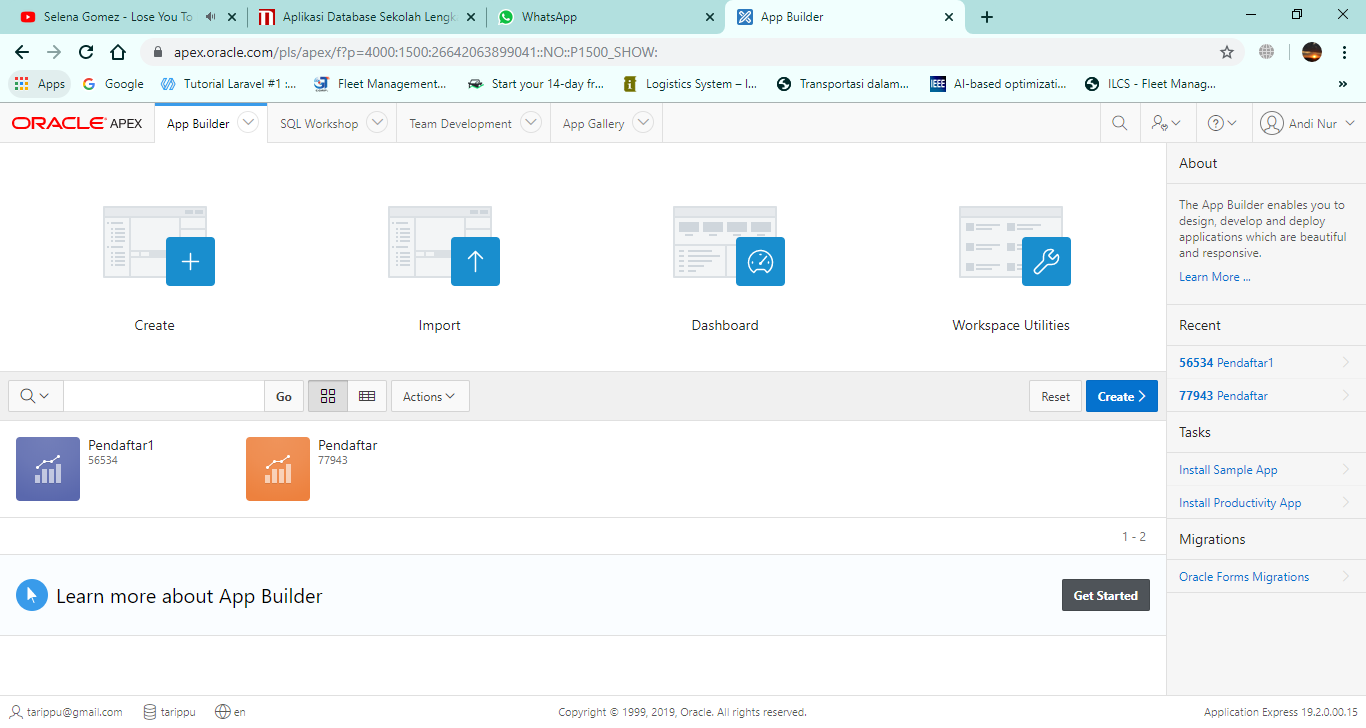
\includegraphics[width=10cm]{figures/4.PNG}
        \caption{Create}
    \end{figure}
    
    \item Setelah masuk ke create an application pilih "From a File"
    \begin{figure}[!htbp]
        \centering
        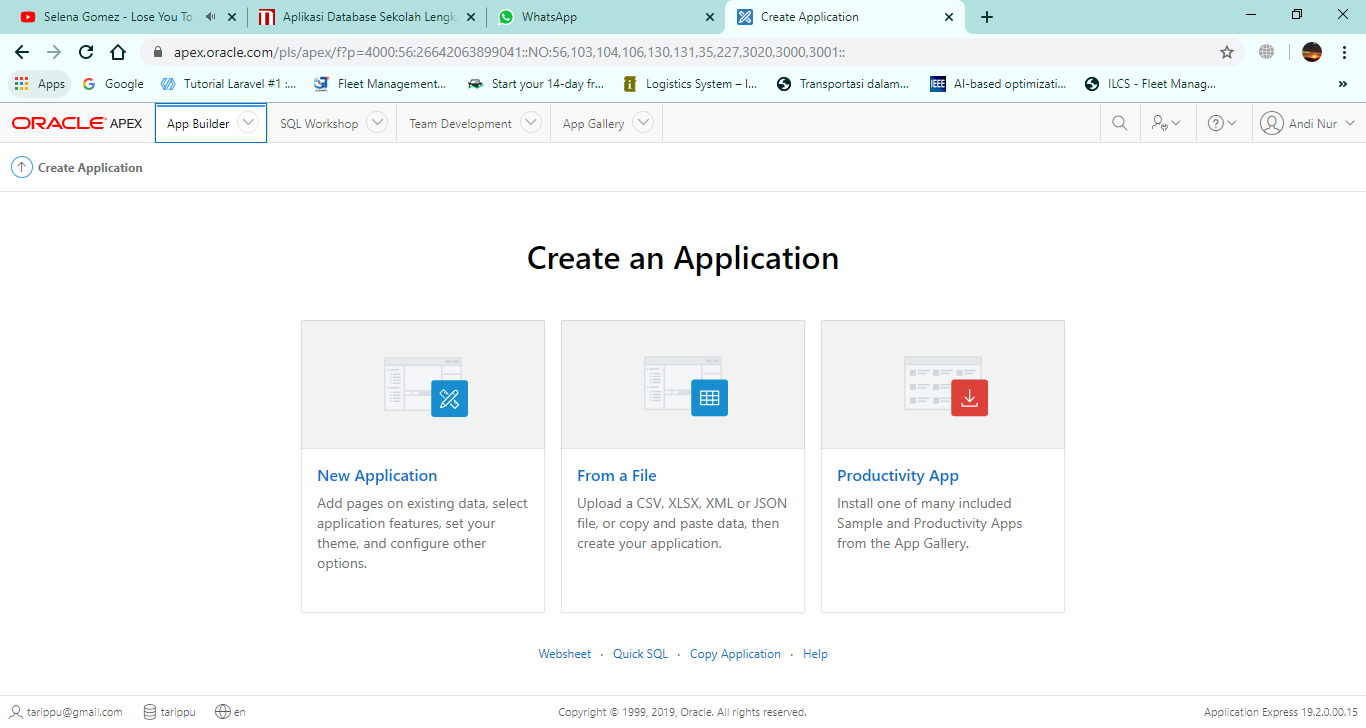
\includegraphics[width=10cm]{figures/5.PNG}
        \caption{From a file}
    \end{figure}
    
    \newpage
    
    \item Drag and drop file CSV data mahasiswa nya. 
    \begin{figure}[!htbp]
        \centering
        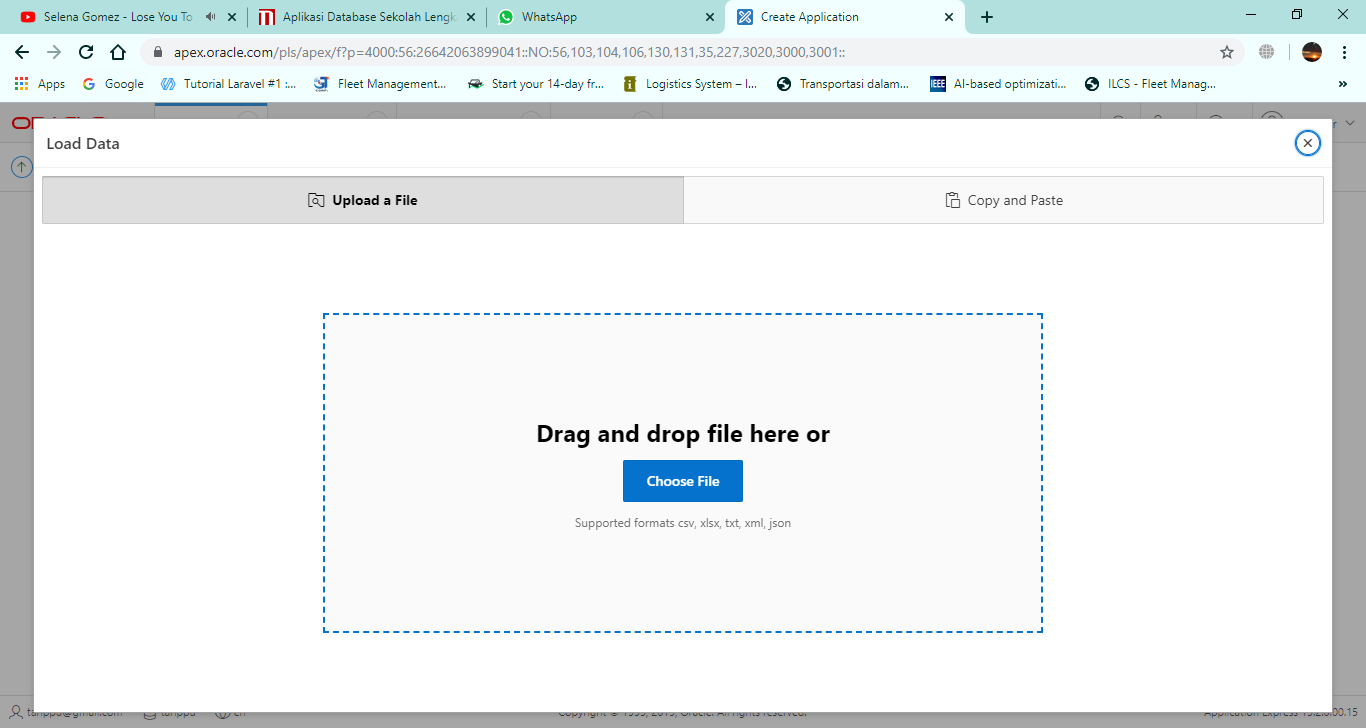
\includegraphics[width=10cm]{figures/6.PNG}
        \caption{Upload data}
    \end{figure}
    
    \item Isi table name, dengan nama MAHASISWA. lalu klik secara otomatis error table namenya akan terisi. klik configure disebelah kanan. 
    \begin{figure}[!htbp]
        \centering
        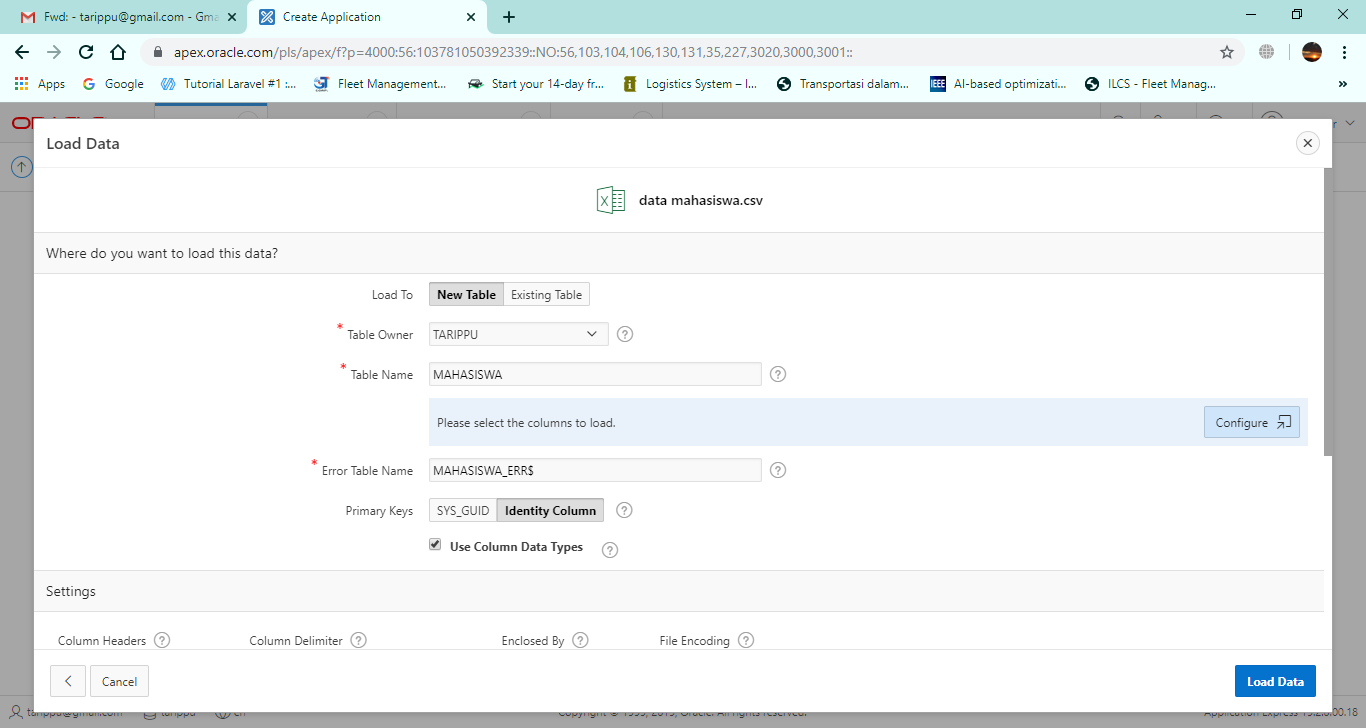
\includegraphics[width=10cm]{figures/8.PNG}
        \caption{Load data}
    \end{figure}
    
    \newpage
    
    \item Setelah muncul isi data dan tidak ada yang error. Klik save changes
    \begin{figure}[!htbp]
        \centering
        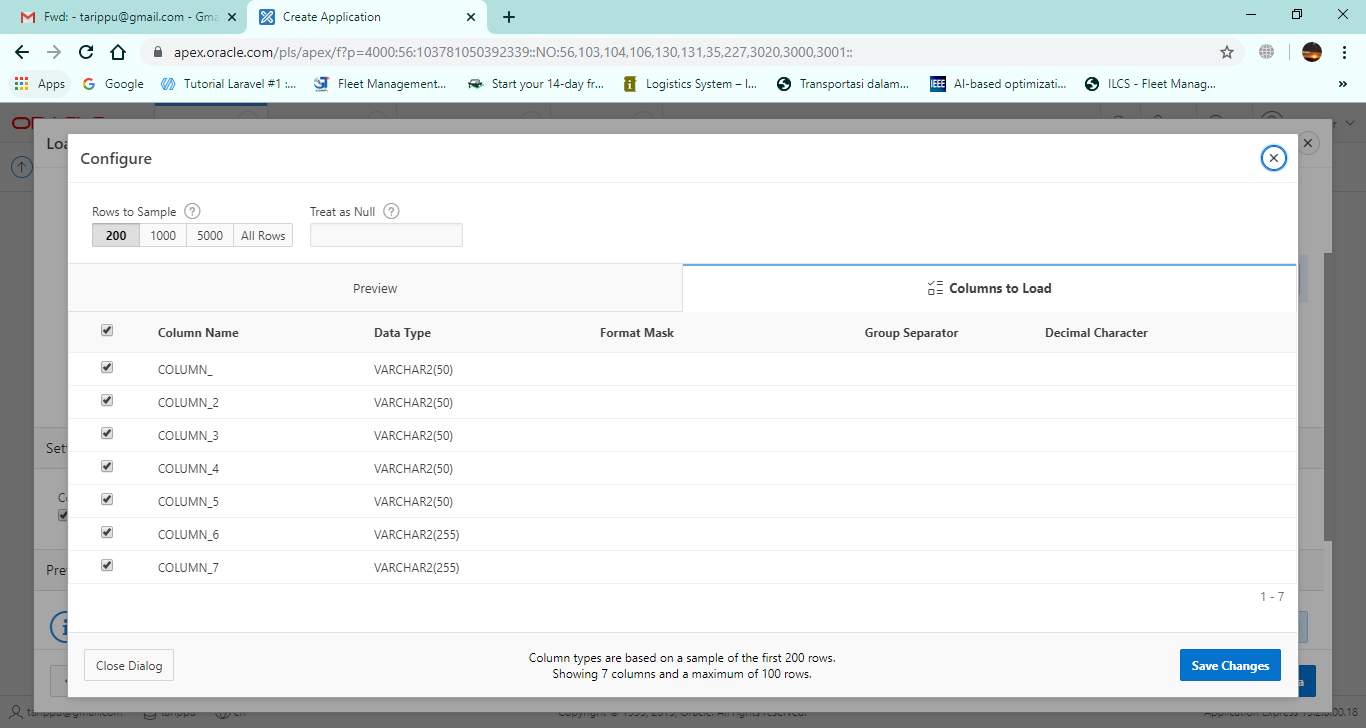
\includegraphics[width=10cm]{figures/9.PNG}
        \caption{Configure}
    \end{figure}

    \item Lalu akan kembali ke tampilan load data. Klik load data Maka akan muncul jumlah rows pada table yg sudah di created. Lalu klik create application
    \begin{figure}[!htbp]
        \centering
        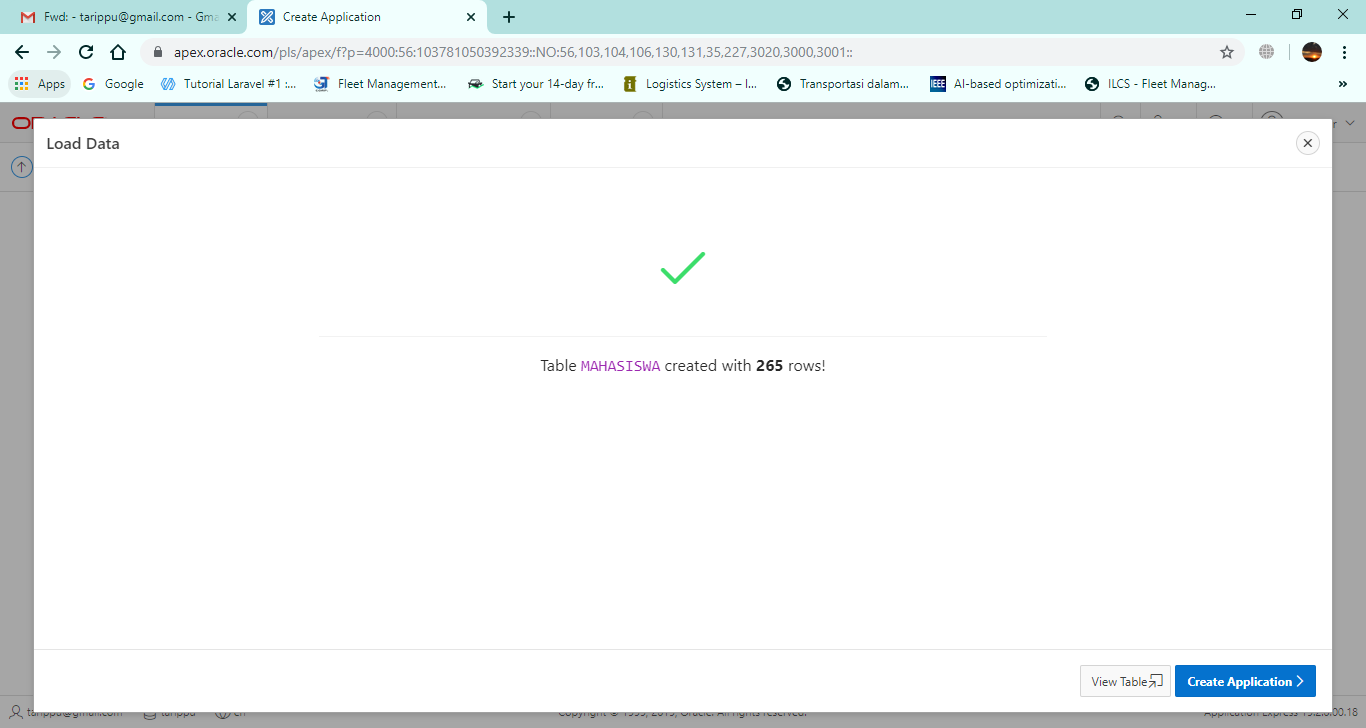
\includegraphics[width=10cm]{figures/10.PNG}
        \caption{Load data}
    \end{figure}
    
    \newpage
    
    \item Maka akan muncul tampilan berikut
    \begin{figure}[!htbp]
        \centering
        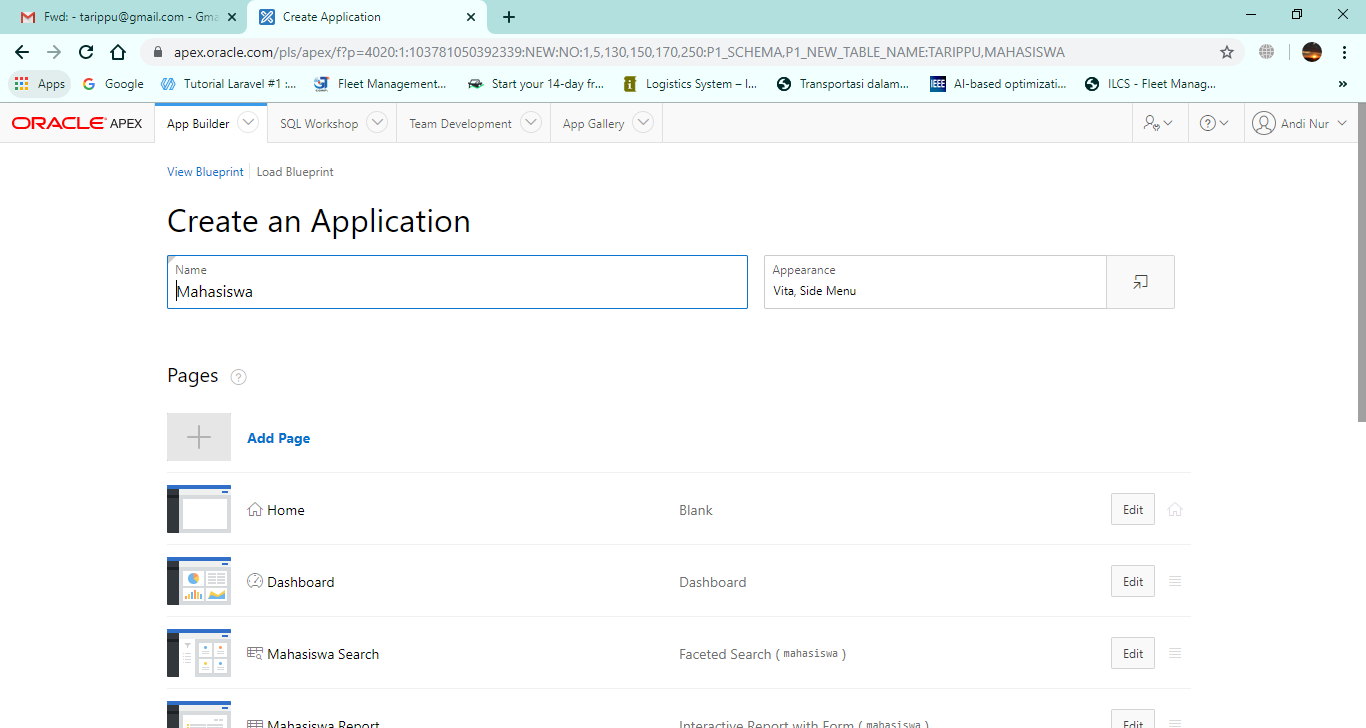
\includegraphics[width=10cm]{figures/11.PNG}
    \end{figure}
    \begin{figure}[!htbp]
        \centering
        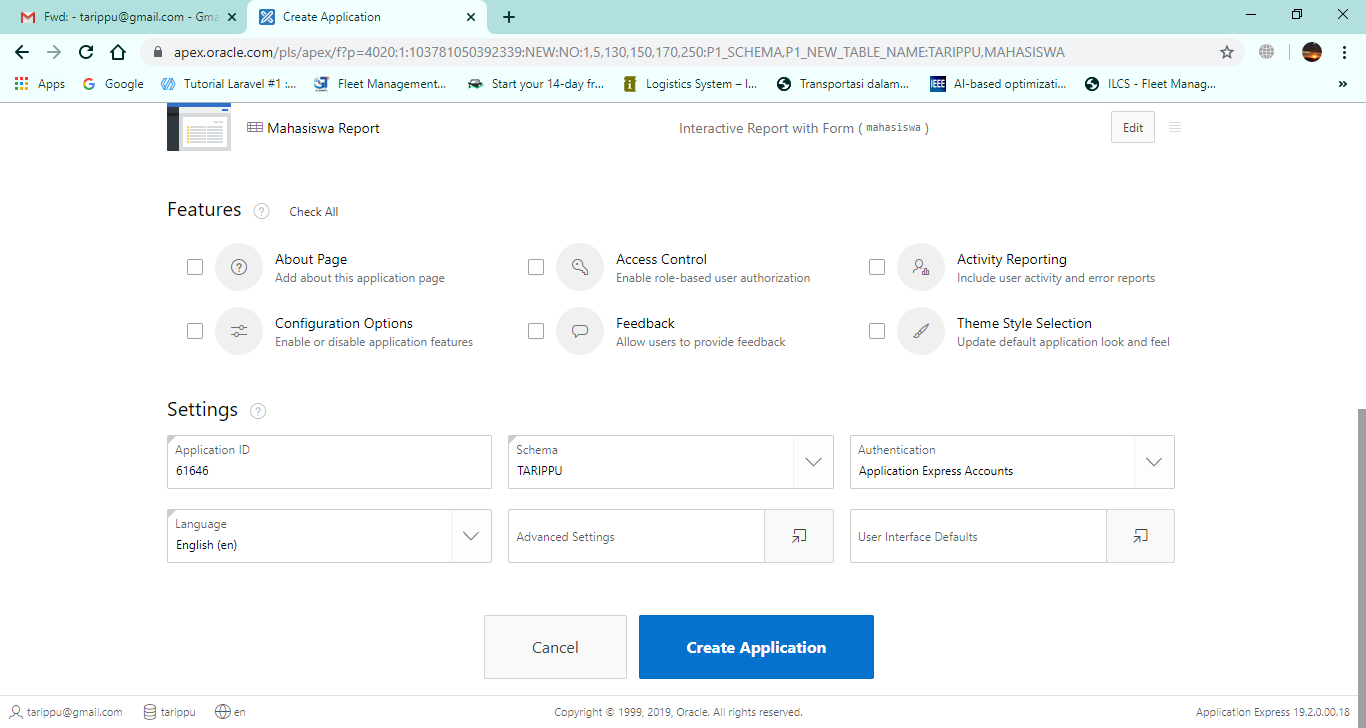
\includegraphics[width=10cm]{figures/12.PNG}
        \caption{Create application}
    \end{figure}
    
    \item Klik Run Application 
     \begin{figure}[!htbp]
        \centering
        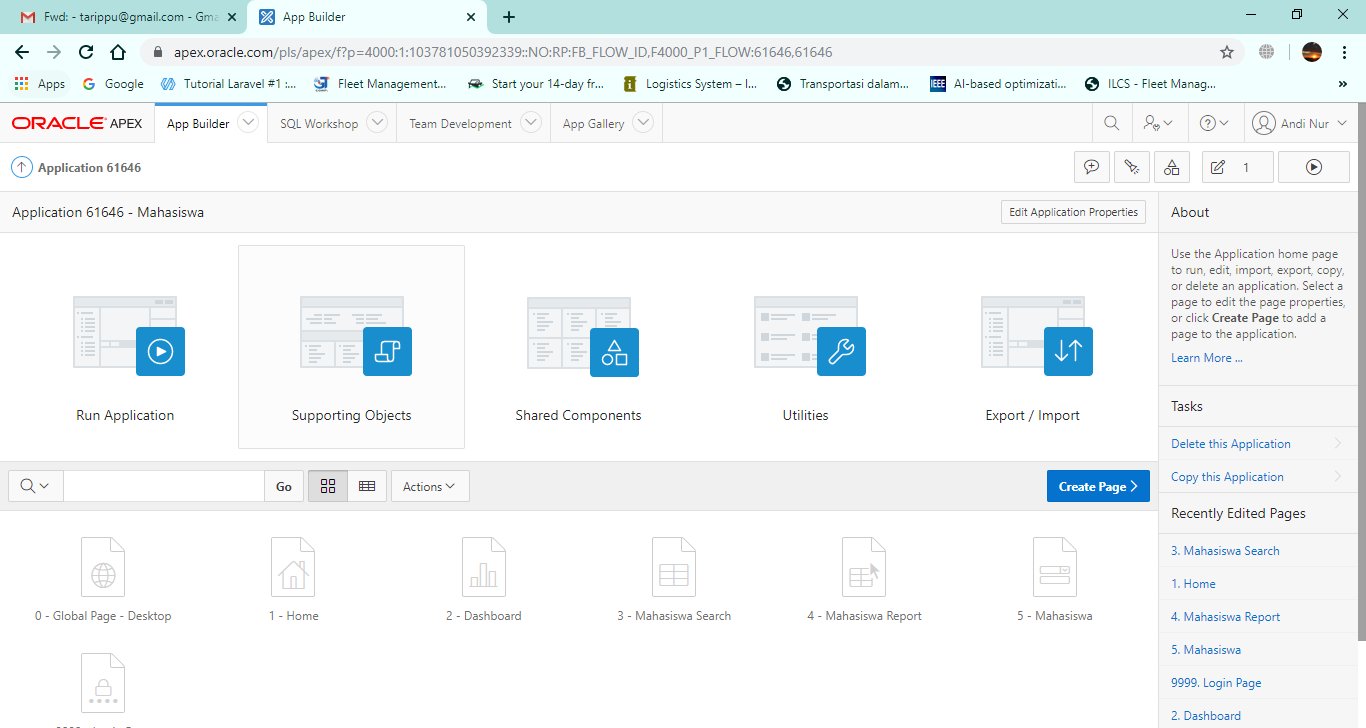
\includegraphics[width=10cm]{figures/13.PNG}
        \caption{Run Application}
    \end{figure}
    
    \item Tampilan berikut adalah tampilan login dari aplikasi mahasiswa yang sudah dibuat. Login masukkan username dan password dari account apex.
     \begin{figure}[!htbp]
        \centering
        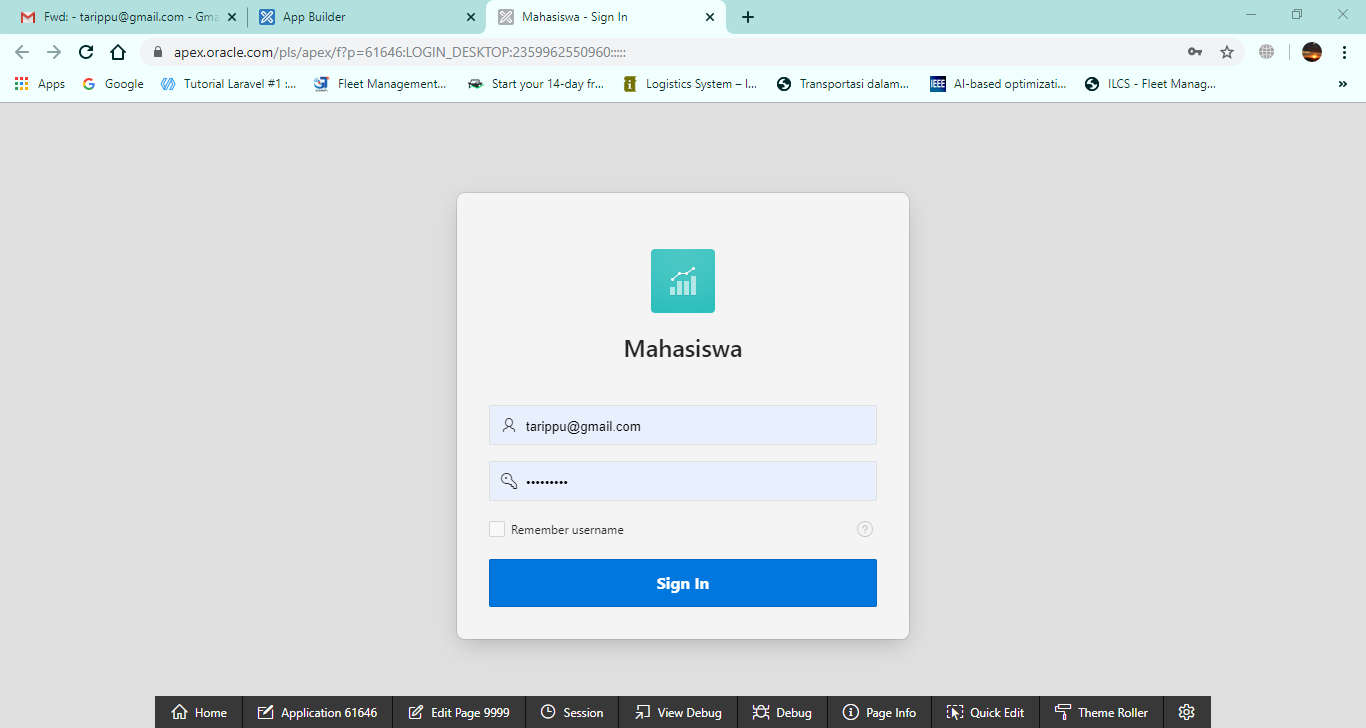
\includegraphics[width=10cm]{figures/14.PNG}
        \caption{Login aplikasi}
    \end{figure}
    
    \item Setelah berhasil login ke aplikasi. Akan muncul tampilan dari aplikasi yang kita buat menggunakan APEX seperti berikut. Aplikasi mahasiswa sudah berhasil dibuat.
    \begin{figure}[!htbp]
        \centering
        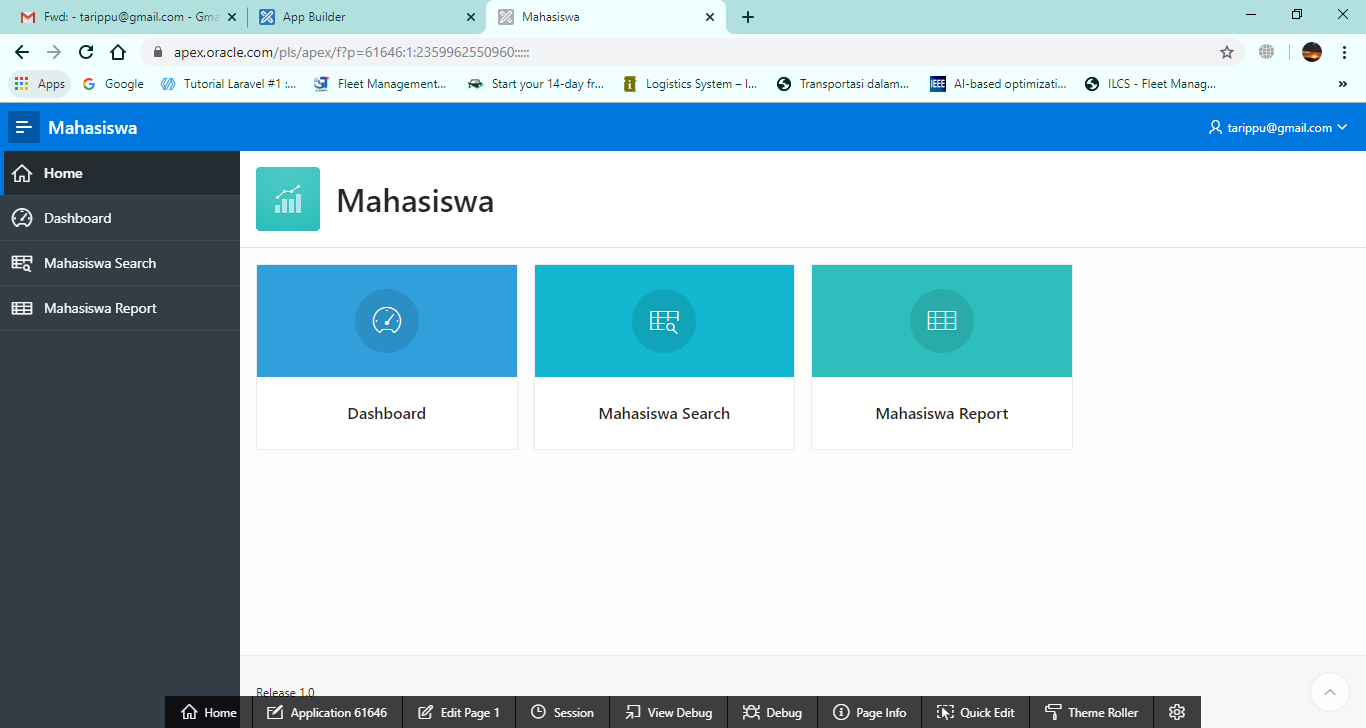
\includegraphics[width=10cm]{figures/15.PNG}
        \caption{Tampilan aplikasi}
    \end{figure}
    
    \newpage
    
    \item Untuk mengecek data mahasiswa pada aplikasi ada pilihan Mahasiswa search, dan mahasiswa report 
     \begin{figure}[!htbp]
        \centering
        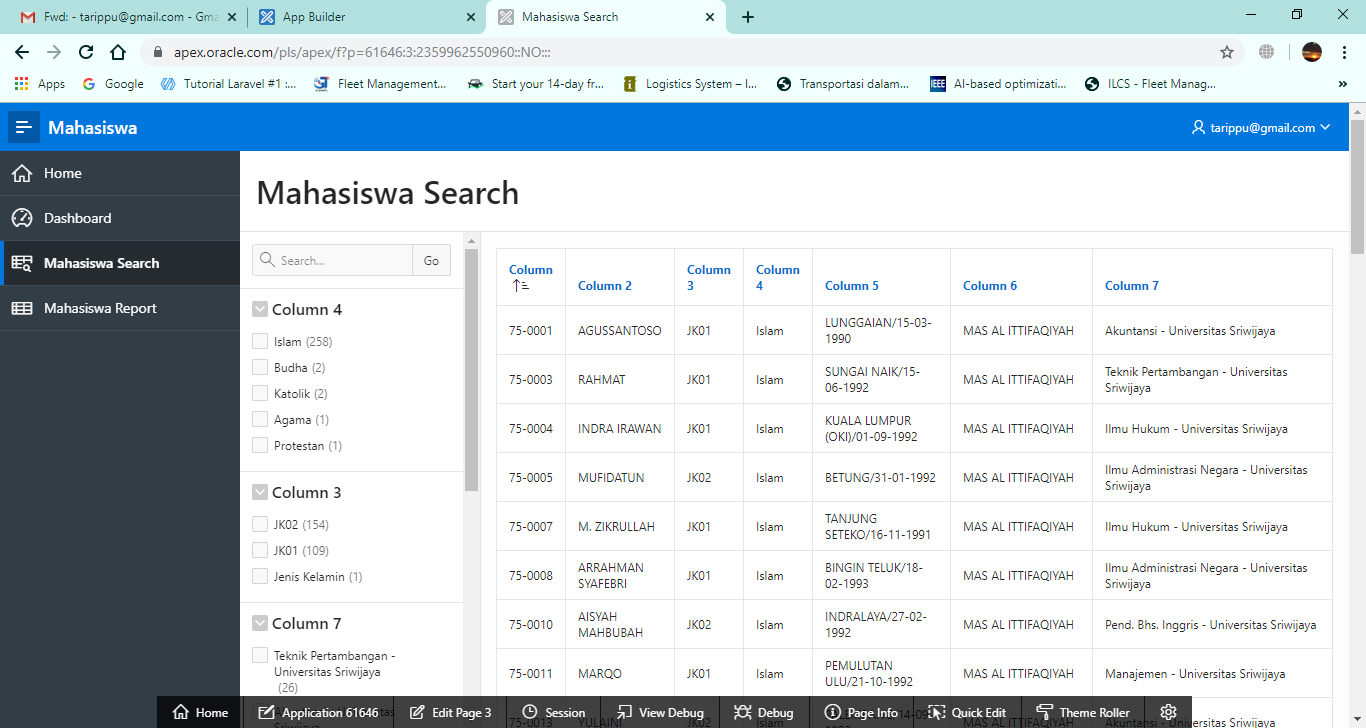
\includegraphics[width=10cm]{figures/17.PNG}
        \caption{rows created}
    \end{figure}
    
    \item Untuk menambahkan table atau ingin mengubah data yg sudah ada pada aplikasi dapat di lakukan pada SQL Commands. 
    
    \section{Account APEX}
    \item WORKSPACE : tarippu
    \item USERNAME  : tarippu@gmail.com
    \item PASS      : taritari2
\end{itemize}
